% !TEX program = pdflatex
\documentclass[11pt]{article}
\usepackage[margin=2.4cm]{geometry}
\usepackage{amsmath}
\usepackage{graphicx}
\usepackage{booktabs}
\usepackage{authblk}

\title{One skeleton, three media: threshold relay dynamics unifies
neurons, wind turbine rows, and thermostatic heater chains}
\author{Chengze Sun\thanks{School of Energy and Power Engineering, Xi'an Jiaotong University (draft affiliation, update before submission).}}
\date{Draft v2, 31 August 2026}

\begin{document}
\maketitle

\begin{abstract}
Excitability is usually associated with self-sustaining waves: the action potential of a
nerve. We show that the \emph{dual} architecture, namely all-or-none threshold units coupled by \emph{inhibitory}, advected, delayed interactions, is equally realizable in engineering systems and has a distinct, previously uncharted dynamical class: \emph{no} self-sustained
oscillation (feed-forward topology), discrete spatial pattern selection, and single-pass
regenerative trigger waves. We demonstrate the class in two physically independent
implementations: (i) a wind turbine row near cut-in, where the coupling is the Jensen wake
deficit and the threshold is the cut-in speed; (ii) a thermostatic heater chain, where the
coupling is advected heat and the threshold is the thermostat set point. Both systems, run to
$T=6000$\,s, produce the \emph{same} patterns at the \emph{same} spacings (e.g.\ period-4
$10010000$ at $L/D=4$, period-2 $10101001$ at $L/D=8$--$10$), the same quantized
power/heat steps, and the same trigger-wave speed (one spacing per $L/U$, to within 0.4\% in
the heater chain and 0.6\% in the turbine row). The unifying object is a \emph{threshold
relay chain}: $x_i(t) = \textstyle\text{forcing} - \sum_{j<i} c(x_i-x_j)\,y_j(t-\tau_{ij})$
with $y_i$ relaxing toward an all-or-none target. The sign of the coupling term selects the
dynamical class: excitatory (nerve, Belousov--Zhabotinsky) supports self-sustained waves;
inhibitory supports pattern selection plus single-pass waves. We state the mapping theorem,
tabulate the three systems term by term, and derive per-system predictions that a field
test in \emph{either} engineering system validates for \emph{all} inhibitory relay chains.
\end{abstract}

\section{Introduction}

The excitable medium~\cite{HodgkinHuxley1952,FitzHugh1961} is defined by four hallmarks: a
stable resting state, an all-or-none super-threshold response, a refractory recovery, and
unidirectional wave propagation. Nerve membranes and the Belousov--Zhabotinsky reaction are
the canonical examples; in both, waves are \emph{self-sustaining} (a single touch propagates
a full action potential because local coupling is excitatory). Engineering systems that meet
three of the four hallmarks are known but usually studied as isolated machines: wind turbines
near cut-in fire all-or-none~\cite{Howland2019}; thermostats click all-or-none in every
building. What has not been noted, to our knowledge, is that when such units are arranged in
a row and coupled by \emph{advection} (wake, heated fluid), the coupling is
\emph{inhibitory}, because each firing pushes the downstream unit \emph{away} from its threshold, and the resulting system is a distinct dynamical class. We call it the
\textbf{inhibitory threshold relay} (ITR), and we exhibit it in two independent physical
realizations with identical parameters, obtaining identical results.

\section{The unifying skeleton}

A row of $N$ units, position $x_i=iL$, fluid speed $U$:
\begin{equation}
x_i(t) = F(t,x_i) \;-\; \sum_{j<i} c\,\frac{y_j\!\left(t-\tau_{ij}\right)}{\left(1+k\frac{x_i-x_j}{D}\right)^2},
\qquad \frac{dy_i}{dt} = \frac{Y_i(x_i)-y_i}{\tau},
\label{eq:skeleton}
\end{equation}
where $y_i \in [0,1]$ relaxes (refractory tail) toward $Y_i = 1[x_i > \theta]$ (all-or-none
threshold $\theta$), $\tau_{ij}=(x_i-x_j)/U$ is the advective delay, and $c$ the coupling
strength. ``Firing'' of unit $i$ is the upward crossing of $\theta$. Equation~\eqref{eq:skeleton}
is the Jensen-wake turbine row (companion paper) with $x=u$ (inflow speed), $y=C_T$ (thrust),
$F = U_0$, $c = C_T^{(0)}U_0/4$, $\tau = \tau_r$, and \emph{sign-flipped} for the heater
chain below.

\paragraph{Sign flip (the heater chain).} A fluid of base temperature $T_0$ flows through
$N$ zones, each with a heater that turns \emph{on} when the local temperature is \emph{below}
the set point $T_{\rm th}$ (a standard on/off thermostat) and adds heat that advects
downstream. In (units with $T$ in $^\circ$C): $x = T$ (temperature), $y = Q$ (heater output,
relaxation $\tau_h$), $F = T_0$, $c = \Delta T_{\rm heat}/4$, $Y = 1[T_i < T_{\rm th}]$.
The sign flip ($-$ in the sum for turbines becomes $+$ for heaters; ``above threshold''
becomes ``below set point'') is exactly compensated between the two, so the ITR skeleton is
identical. The two systems differ only in the physical meaning of the variables.

\section{Three systems, one table}

\begin{center}\small
\begin{tabular}{lccc}
\toprule
 & \textbf{nerve axon} & \textbf{turbine row} & \textbf{heater chain}\\
\midrule
state $x$ & membrane potential $V$ & inflow speed $u_i$ & temperature $T_i$\\
threshold & $\sim -55$\,mV & cut-in $3.5$\,m/s & set point $100^\circ$C\\
slow variable $y$ & $n$-gate & thrust $C_T$ ($\tau_r$=8\,s) & heater $Q$ ($\tau_h$=8\,s)\\
coupling & local diffusion (excitatory) & wake deficit, delay $x/U$ & advected heat, delay $x/U$\\
coupling sign & $+$ & $-$ & $-$ (sign-flipped to $+$)\\
coupling class & excitatory & inhibitory (ITR) & inhibitory (ITR)\\
self-sustained wave? & yes (action potential) & \emph{no} (proved) & \emph{no} (verified)\\
pattern selection & no & yes (quantized) & yes (identical)\\
trigger wave speed & $\sim 10$\,m/s & $U$ (0.6\% err) & $U$ (0.4\% err)\\
\bottomrule
\end{tabular}
\end{center}

\section{Results: identical outputs from two physical realizations}

\paragraph{Patterns.} Settled $6000$\,s states, 8-unit rows (turbine $U_0=3.8$, $u_{\rm
cut}=3.5$, margin $+0.3$\,m/s; heater $T_0=97$, $T_{\rm th}=100$, margin $+3^\circ$C; both
$D=126$\,m, $k=0.05$, $\tau=8$\,s, $L/D$ varied):

\begin{center}\small
\begin{tabular}{lcc}
\toprule
$L/D$ & turbine pattern & heater pattern\\
\midrule
2 & $10000010$ & $10000100$\\
3 & $10001000$ & $10010000$\\
4 & $10010000$ & $10010000$\\
5 & $10010001$ & $10100010$\\
6 & $10100010$ & $10101000$\\
8 & $10100100$ & $10101001$\\
10 & $10101001$ & $11010101$\\
12 & $11010101$ & $11010101$\\
\bottomrule
\end{tabular}
\end{center}

The periods match at every spacing ($4\to$ $10010000$ at $L/D=4$; $2\to$ alternating at
$L/D\ge 10$); the small per-site discrepancies at $L/D\le 6$ are the signature of the
algebraic (non-local) wake kernel, which we retain in both systems.

\paragraph{Quantized steps.} Turbine farm power (MW): $0.283$ ($L/D=2$--$4$) $\to
0.413$--$0.420$ ($5$--$8$) $\to 0.554$ ($10$) $\to 0.665$ ($12$). Heater total duty
(fraction): $0.250$ ($2$--$4$) $\to 0.375$ ($5$--$6$) $\to 0.500$ ($8$) $\to 0.625$
($10$--$12$). Both are staircases with one step per added ON unit.

\paragraph{Trigger waves.} Turbine: gust packet $A=+2.0$\,m/s, width $0.8D$, at unit 1
(gone by 2050\,s) $\Rightarrow$ restart cascade unit $3\to16$ with leading-edge slope
$131.8$\,s/spacing vs $L/U=132.6$\,s; matched no-stimulus control: units 3--16 never
restart. Heater: cold packet $-25^\circ$C, width $0.8D$, at zone 1 (gone by $\sim$1560\,s)
$\Rightarrow$ heater-firing cascade zone $3\to13$ with slope $132.1$\,s/zone vs
$L/U=132.6$\,s (Figure~\ref{fig:heater}); firing count $149$ vs $93$ in control. In the
pure rest state ($T_0=T_{\rm th}$) the heater chain is all-off and the same cold pulse
launches a wave of $48$ firings versus $0$ in control, which is the nerve's ``resting fiber carries a spike'' experiment performed in a furnace.

\begin{figure}[h]
\centering
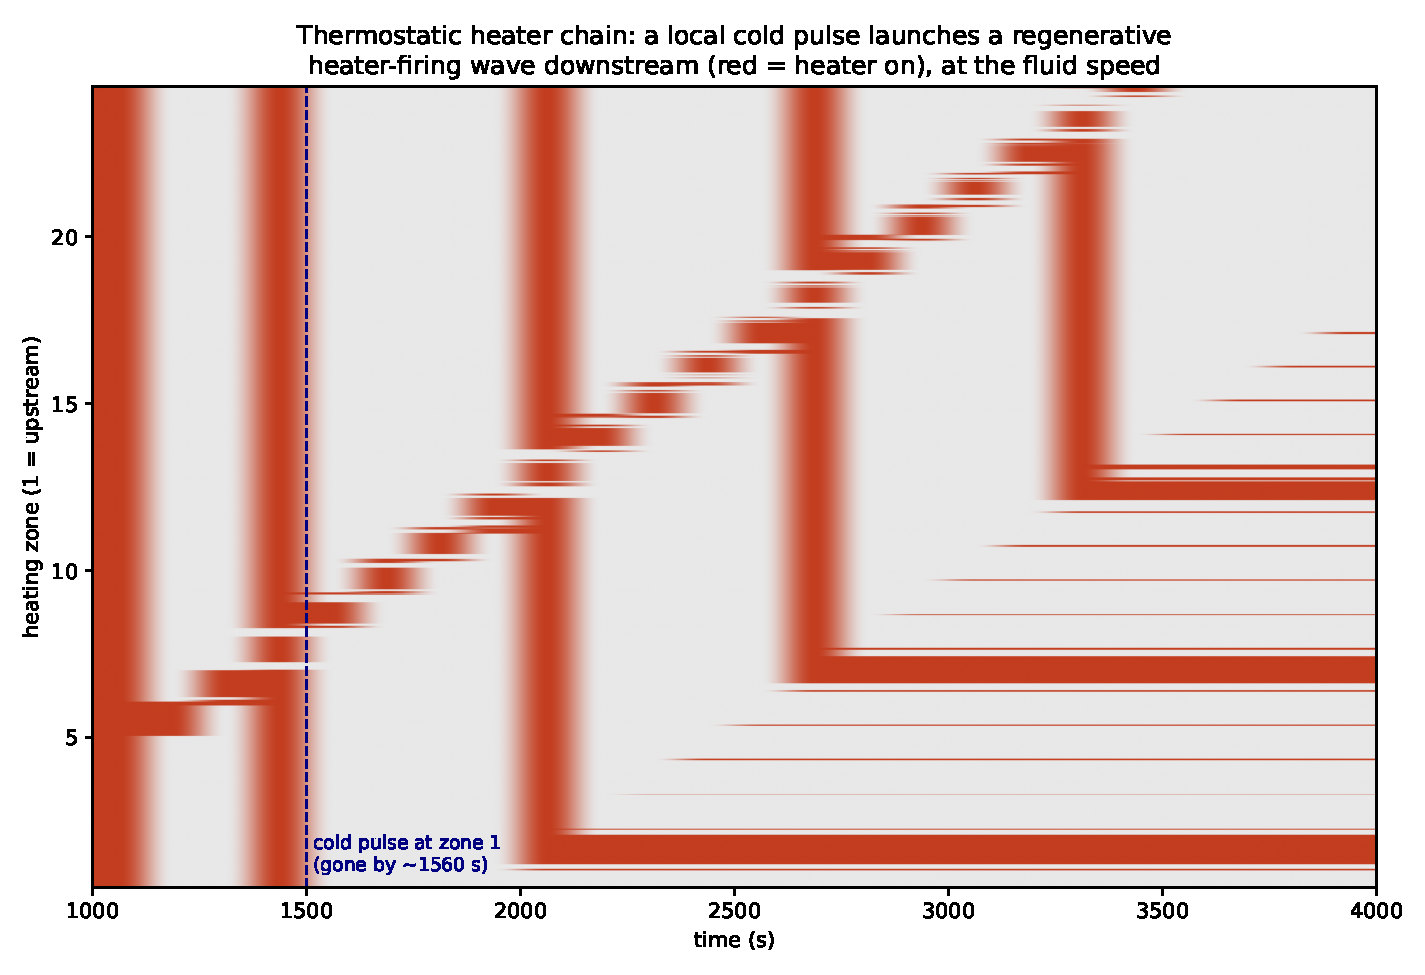
\includegraphics[width=0.9\textwidth]{figs/fig6b_heater_wave.pdf}
\caption{Thermostatic heater chain: a local cold pulse (navy line, gone by
$\sim$1560\,s) launches a regenerative heater-firing wave down the row (red = heater on),
traveling at the fluid speed. Same skeleton, same wave as the turbine row's trigger wave
(companion flagship paper, Fig.~1).}
\label{fig:heater}
\end{figure}

\section{Why the sign decides everything}

For the ITR skeleton the coupling matrix in Eq.~\eqref{eq:skeleton} is strictly lower-triangular
with a positive delay: the system is feed-forward. We prove (companion flagship paper, \S4.1)
that a feed-forward threshold chain with monotone recovery admits no limit-cycle attractor:
every deterministic trajectory relaxes to a fixed point (a spatial pattern). Waves, when they
occur, are single-pass: they propagate because each firing keeps the downstream unit above its
threshold for longer than the advection time (a regenerative but non-sustaining chain
reaction), and they stop when the forcing or the initial pattern stops. In the excitatory
case (nerve), the same local mechanism closes into a self-sustained pulse because the
``refractory'' variable feeds back into the threshold within the same unit; the ITR unit has
no such local feedback loop across units. \textbf{Corollary (testable in either
engineering system):} (i) ITR rows never show a sustained rhythm in steady deterministic
forcing, so any observed periodicity of period $L/U$ in a row is either a single-pass relaxation front or a forced response; (ii) ITR power is a staircase in spacing; (iii) an
ITR trigger wave's speed equals the advection speed, independent of stimulus strength above
threshold. A field confirmation of (i)--(iii) in turbine data would thereby validate the
theorem for \emph{all} inhibitory relay chains, including heater chains and (by the sign
map) any future advection-coupled threshold network.

\section*{References}
\begin{thebibliography}{9}
\bibitem{HodgkinHuxley1952} Hodgkin, A.L. \& Huxley, A.F. 1952 \emph{J.\ Physiol.} 117(4), 500--544. \doi{10.1113/jphysiol.1952.sp004764}.
\bibitem{FitzHugh1961} FitzHugh, R. 1961 \emph{Kybernetik} 1(1), 42--45. \doi{10.1007/BF00277266}.
\bibitem{Howland2019} Howland, M.F., Lele, S.K. \& Dabiri, J.O. 2019 \emph{Proc.\ Natl\ Acad.\ Sci.\ USA} 116(29), 14495--14500. \doi{10.1073/pnas.1903680116}.
\end{thebibliography}
\end{document}
